%%%%%%%%%%%%%%%%%%%%%%%%%%%%%%%%%%%%%%%%%%%%%%%%%%%%%%%%%%%%%%%%%
% Tese de Doutorado / Dept. Fisica, CFM, UFSC                   %
% Lacerda@CórregoGrande - Jan/2018                              %
%%%%%%%%%%%%%%%%%%%%%%%%%%%%%%%%%%%%%%%%%%%%%%%%%%%%%%%%%%%%%%%%%

%:::::::::::::::::::::::::::::::::::::::::::::::::::::::::::::::%
%                                                               %
%                   Anexo EmLinesDataCube                       %
%                                                               %
%:::::::::::::::::::::::::::::::::::::::::::::::::::::::::::::::%

\chapter{Organizando os ajustes nebulares com o EmLinesDataCube}
\label{apendice:EmLinesDataCube}

Feitas as medidas dos fluxos integrados das linhas de emissão, conforme descrito na Seção \ref{sec:sample:eml}, temos o arcabouço para calcularmos propriedades nebulares. Escrevi um objeto em \pyt (cujo nome titula esta seção) que, além de organizar os resultados provenientes do programa de medida das linhas de emissão, calcula o coeficiente de extinção para as regiões nebulares ($\tauVN$), larguras equivalentes das linhas, assim como os erros propagados em cada cálculo. Esse objeto foi adicionado ao PyCASSO para facilitar a utilização dos demais membros do projeto. Com esse módulo fica fácil acessar as medidas dos fluxos integrados, a posição central, amplitudes e largura das principais linhas de emissão, coeficientes para reconstrução do contínuo ao redor de cada linha de emissão, os erros nestas medidas, as propriedades mencionadas anteriormente e seus erros propagados.


\section{Propriedades calculadas}
\label{apendice:EmLinesDataCube:props}

\subsection{Extinção estimada através do decremento de Balmer}
\label{apendice:EmLinesDataCube:props:tauvneb}
Em um modelo que assume que entre o observador e a fonte de energia existe uma camada difusa, como uma cortina, que extingue a luz diferentemente em cada comprimento de onda, temos:
\begin{equation}
	F_\lambda^{obs} = F_\lambda^{int} e^{-\tau_\lambda}
    \label{eq:extin}
\end{equation}
\noindent onde $F_\lambda^{int}$ é o fluxo intrínseco ($F_\lambda^{obs}$, o observado) em cada comprimento de onda, $\tau_\lambda$ é a profundidade óptica para o comprimento de onda $\lambda$ (neste trabalho também o chamamos de coeficiente de extinção). O modelo de extinção de \citet{CCM1989a} nos dá uma calibração empírica da razão entre os coeficientes de extinção em um comprimento de onda e na banda V. Com isso podemos desenvolver \eqref{eq:extin} de maneira que possamos escrever uma equação para $\tau_V$:
\begin{eqnarray}
   F_\lambda^{obs} &=& F_\lambda^{int} e^{-(\frac{\tau_\lambda}{\tauV}) \tauV} \\
   q_\lambda &\equiv& \frac{\tau_\lambda}{\tauV} \\
   F_\lambda^{obs} &=& F_\lambda^{int} e^{-q_\lambda \tauV} \\
   \frac{F_\lambda^{obs}}{F_{\lambda^\prime}^{obs}} &=& \
 \frac{F_\lambda^{int} e^{-q_\lambda \tauV}}{F_{\lambda^\prime}^{int} e^{-q_{\lambda^\prime} \tauV}} \\
   \ln \left(\frac{F_\lambda^{obs}}{F_{\lambda^\prime}^{obs}}\right) &=& \
 \tauV (q_{\lambda^\prime} - q_\lambda) \ln \left(\frac{F_\lambda^{int}}{F_{\lambda^\prime}^{int}}\right) \\
   \tauV &=& \frac{1}{(q_{\lambda^\prime} - q_\lambda)} \left[\ln \
 \left(\frac{F_\lambda^{obs}}{F_{\lambda^\prime}^{obs}}\right) - \
 \ln \left(\frac{F_\lambda^{int}}{F_{\lambda^\prime}^{int}}\right)\right]
 \label{eq:tauV}
\end{eqnarray}
\noindent Nessa equação, os $q_\lambda$ são provenientes da curva de extinção adotada.

Utilizando \eqref{eq:tauV} podemos calcular qual o coeficiente de extinção para essas regiões nebulares. Para este cálculo utilizamos o fato de que a razão entre os fluxos intrínsecos das duas primeiras linhas da série de Balmer, \Ha e \Hb, varia muito um pouco com a metalicidade, a densidade e a temperatura. Usamos aqui esse valor como constante e igual a $2.86$ \citep[densidade eletrônica de $n = 100\ cm^{-3}$ e temperatura eletrônica $T_e = 10^4$ K; ][]{Osterbrock.Ferland.2006a}. Tambem utilizamos $q_{\Ha}  = 0.81775$ e $q_{\Hb} = 1.16427$ (valores da calibração empírica feita por \citeauthor{CCM1989a}). Com isso temos:
\begin{equation}
	\tauVN = 2.886\ \ln \left( \frac{F_{\Ha}^{obs}/F_{\Hb}^{obs}}{2.86} \right).
\end{equation}

O valor de $\tauVN$ varia tipicamente entre 0.6 e 0.65 (média e mediana) nas regiões aqui estudadas (ver também Seção \ref{apendice:synvsneb:tauv}).
O erro propagado para $\tauVN$ é:
\begin{eqnarray}
	\tauVN &\equiv& \tauVN(F_{\Ha}^{obs}, F_{\Hb}^{obs}) \\
	\epsilon (\tauVN) &=& \sqrt{\left(\del{\tauVN}{F_{\Ha}^{obs}}\right)^2 \
\epsilon (F_{\Ha}^{obs})^2 + \left(\del{\tauVN}{F_{\Hb}^{obs}}\right)^2 \
\epsilon (F_{\Hb}^{obs})^2 } \\
	\del{\tauVN}{F_{\Ha}^{obs}} &=& \frac{1}{F_{\Ha}^{obs} (q_{\Hb} - q_{\Ha})} \\
	\del{\tauVN}{F_{\Hb}^{obs}} &=& - \frac{1}{F_{\Hb}^{obs} (q_{\Hb} - q_{\Ha})} \\
	\epsilon (\tauVN) &=& \frac{1}{(q_{\Hb} - q_{\Ha})} \
\sqrt{\left(\frac{\epsilon (F_{\Ha}^{obs})}{F_{\Ha}^{obs}}\right)^2 + \
\left(\frac{\epsilon (F_{\Hb}^{obs})}{F_{\Hb}^{obs}}\right)^2 }
	\label{eq:etauneb}
\end{eqnarray}
\noindent Os termos de dentro da raiz em \eqref{eq:etauneb} são o inverso das relações sinal-ruído ($S/N$) de \Ha e \Hb. Como \Hb é sempre a mais ruidosa das duas, podemos aproximar a incerteza em $\tauVN$ por:
\begin{equation}
	\epsilon (\tauVN) \approx \frac{2.886}{(S/N)_{\Hb}}
	\label{eq:etaunebaprox}
\end{equation}
\noindent com valor típico $\sim 0.14$.

\subsection{Cálculo da taxa de formação estelar}
\label{apendice:EmLinesDataCube:props:SFR}
Um dos métodos mais utilizados para medida da SFR recente utiliza a linha de emissão de \Ha. Nesse método assume-se que a formação estelar é constante nos últimos $t$ anos, que deve englobar pelo menos o tempo de vida das estrelas massivas ionizantes, as quais produzem basicamente todos os fótons que geram as linhas de emissão em \Ha.

Nós queremos calibrar $\LHalpha$ como um indicador de SFR usando uma relação linear:
\begin{equation}
	\mathrm{SFR}_{\Ha} = k \times \LHalpha.
	\label{eq:SFRHa}
\end{equation}
\noindent Portanto, nosso trabalho é encontrar $k$. Faremos isso investigando a natureza dos
fótons H-ionizantes.

Chamamos $\Lambda$ o valor total de luz ($l$) que recebemos de estrelas que se formaram $t$ anos atrás. $l(t)$ pode ser qualquer função que descreve a evolução temporal de qualquer fonte radiativa genérica \emph{por unidade de massa formada}\footnote{A expressão {\em massa formada} é aqui utilizada porque quando falamos de sistemas estelares temos que diferenciar o quanto de massa se tornou em estrelas e o quanto ainda continua na forma de estrelas. Isso acontece porque a evolução estelar devolve matéria para o meio interestelar (atrvés de explosão de supernovas, nebulosas planetárias, ventos, etc). Uma SSP pode devolver para o ISM até 50\% de massa durante um tempo de Hubble, dependendo, entre outras coisas, da função de massa inicial ({\em initial mass function}; IMF).} de uma população estelar simples ({\em simple stellar population}; SSP):
\begin{equation}
	\Lambda(t) = \int_0^t l(t')\ \textrm{d}\textrm{M}(t').
	\label{eq:dLambda}
\end{equation}
\noindent Para obter $\Lambda$ nos falta saber como a massa em estrelas cresce no tempo, ou seja, saber como a SFR varia no tempo:
\begin{equation}
	\mathrm{d}\mathrm{M}(t)\ =\ \mathrm{SFR}(t)\ \mathrm{d}t
	\label{eq:dM_t}
\end{equation}

%---------------------------- Figure ----------------------------
\begin{figure}
	\centering
	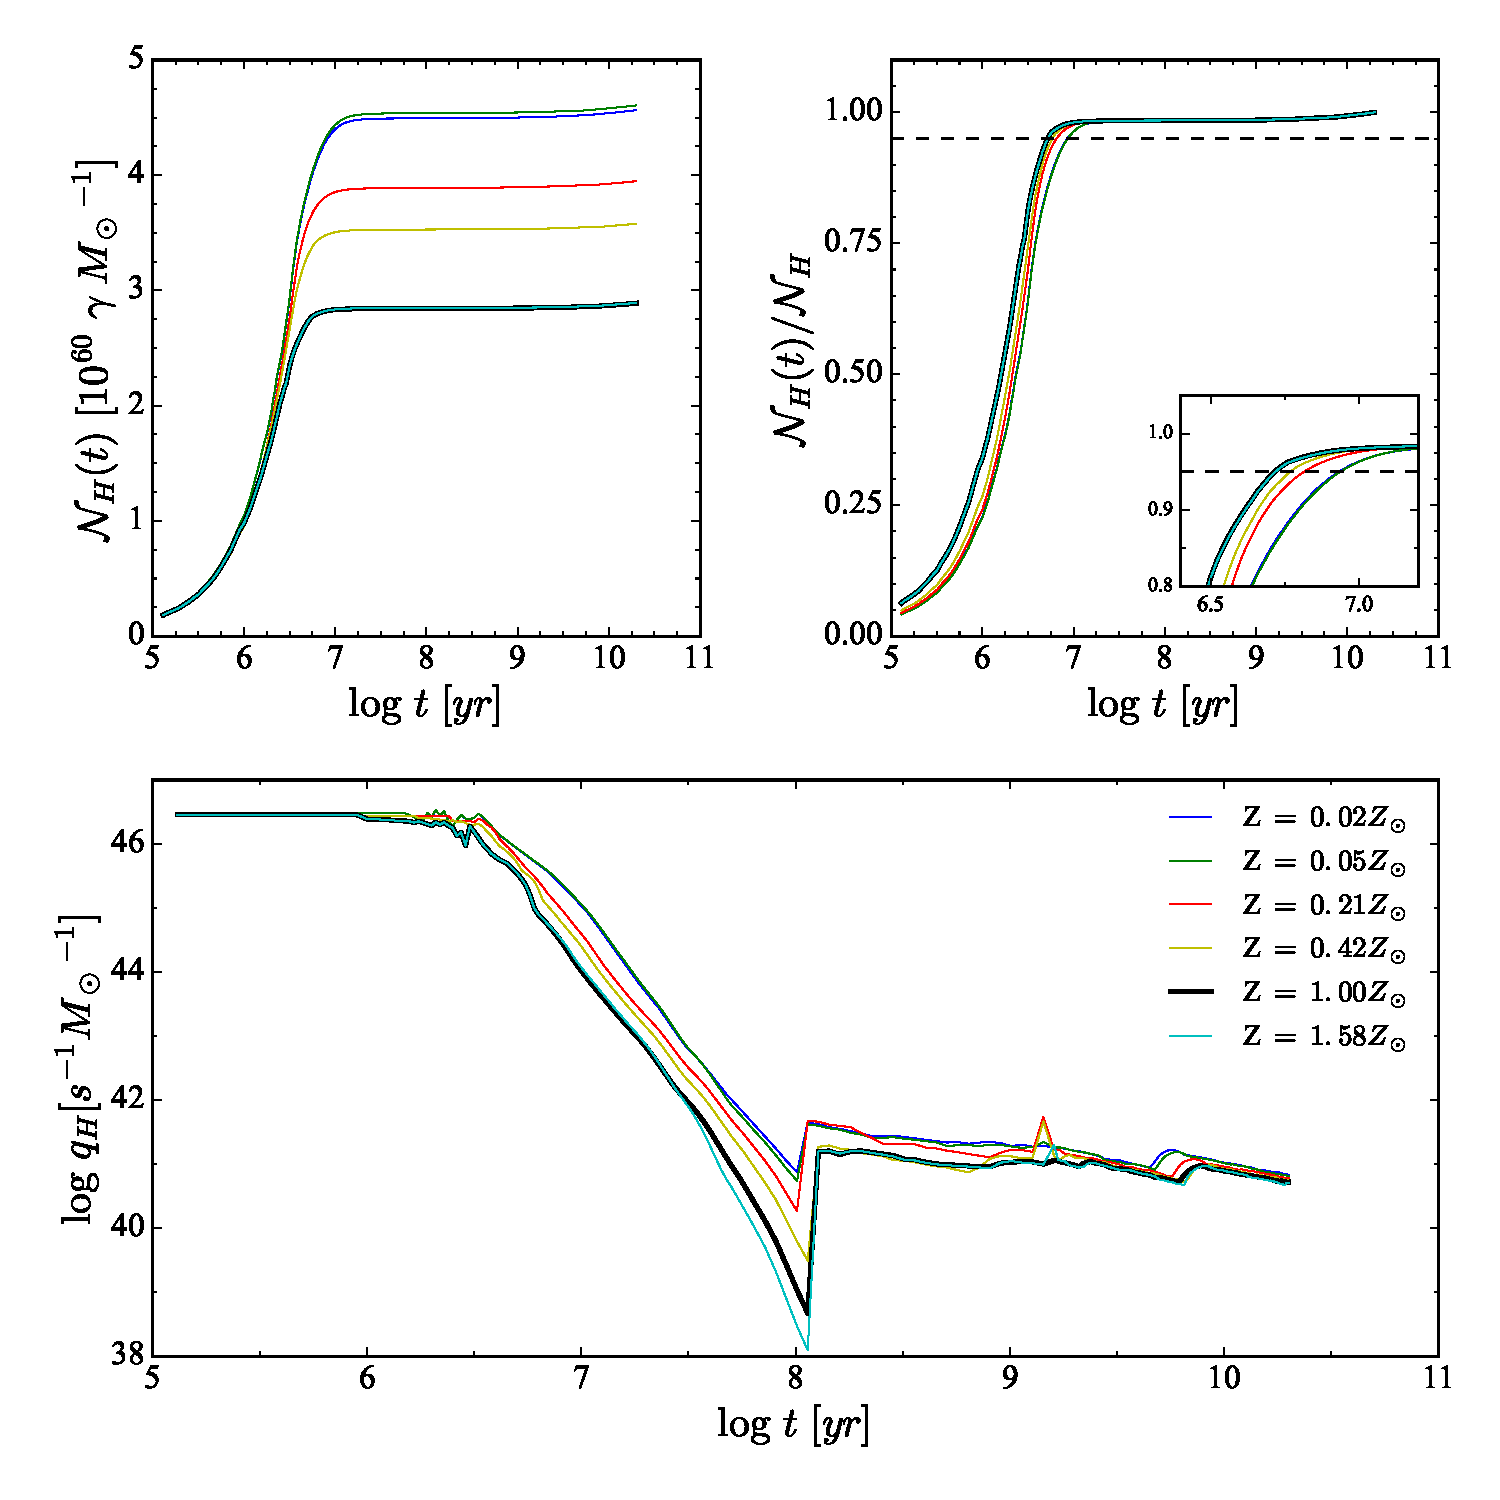
\includegraphics[scale=0.62]{figuras/Nh_logt_metBase_Padova2000_salp.pdf}
	\caption[Evolução temporal do número e da taxa de fótons H-ionizantes em unidades da massa
	formada.]
	{\emph{Painel superior esquerdo}: A	evolução no tempo do número de fótons ($\mathcal{N}_H$) para 6 metalicidades (de 0.02 $Z_\odot$ até 1.58 $Z_\odot$) que compoem nossos modelos de SSP. A linha preta grossa representa a evolução utilizando metalicidade solar. \emph{Painel superior direito}: O mesmo que o \emph{painel superior esquerdo}, contudo normalizado pelo valor total de $\mathcal{N}_H$. A linha pontilhada representa 95\% do total de $\mathcal{N}_H$. Em destaque a região ao redor de 10 milhões de anos. \emph{Painel inferior}: Evolução da taxa de fótons H-ionizantes em unidades da massa formada. Também mostra o valor seguindo o código de cores para as mesmas metalicidades.}
	\label{fig:Nh_qh}
\end{figure}
%---------------------------- Figure ----------------------------

Utilizando \eqref{eq:dM_t} em \eqref{eq:dLambda} e integrando dentro do tempo do Universo ($T_U\ \sim$ 14 bilhões de anos) teremos hoje um total de luz:
\begin{eqnarray}
	\Lambda(t = T_U) &=& \int_0^{T_U} l(t)\ \textrm{d}\textrm{M}(t) \\
	&=& \int_0^{T_U} l(t)\ \mathrm{SFR}(t)\  \textrm{d}t
	\label{eq:Lambda}
\end{eqnarray}
\noindent Assumindo o caso B de recombinação do hidrogênio, um em cada 2.206 fótons ionizantes produzem um fóton de \Ha \citep{Osterbrock.Ferland.2006a}\footnote{Em um volme $\Delta V$ de uma região \hii, o número de recombinações $p + e \rightarrow {\rm H}^0$ por tempo é dado por $n_p n_e \alpha_B({\rm H}^0) \Delta V$, onde $n_e$ e $n_p$ são as densidades eletronica e protônica e $\alpha_B({\rm H}^0)$ é o coeficiente total de recombinações para o caso B. Na Tabela 2.7 de \citet{Osterbrock.Ferland.2006a} temos $\alpha_B({\rm H}^0) = 2.59\times10^{-13}$ recombinações $\times\,cm^3\,s^{-1}$ (para uma temperatura de $10\,000$ K). Durante a cascata de recombinação, alguns dos elétrons passam pela transição $n = 3 \rightarrow 2$, produzindo \Ha. Seja $\alpha_{\Ha}^{eff}({\rm H}^0)$ o coeficiente que conta apenas esse tipo de recombinação. Esse valor não é explicitamente dado no livro de \citet{Osterbrock.Ferland.2006a}, porém eles provém (na Tabela 4.7) o valor eficaz para \Hb ($\alpha_{\Hb}^{eff}({\rm H}^0) = 3.03\times10^{-14}$), juntamente com a razão entre as emissividades $j_{\Ha}/j_{\Hb} = 2.87$. Usando
$$
\frac{ \alpha_{\Ha}^{eff}({\rm H}^0) }{ \alpha_{\Hb}^{eff}({\rm H}^0) } = \frac{ j_{\Ha} / h\nu_{\Ha} }{ j_{\Hb} / h\nu_{\Hb} }
$$
\noindent (onde a razão de energias dos fótons de \Ha e \Hb aparecem porque $j$ mede energia e $\alpha$ mede um número de recombinações), nós finalmente obtemos $\alpha_{\Ha}^{eff}({\rm H}^0) = 1.17\times10^{-13} \, cm^{3}\,s^{-1}$ , ou $0.453 \times \alpha_B({\rm H}^0)$. Em outras palavras, um a cada $1/0.453 = 2.206$ recombinações produz um fóton de \Ha. Considerando a núvem em equilíbrio (o número de fotoionizações se balanceia com o de recombinações) e que a radiação $h\nu > 13.6$ eV não escape da núvem, podemos finalmente dizer que um a cada 2.206 fótons ionizantes produz um fóton \Ha.}. Esse número não varia muito em função da temperatura e da densidade nas regiões \Hii. Portanto:
\begin{equation}
	\LHalpha = h \nu_{\Ha} \frac{\mathrm{Q}_H}{2.206},
	\label{eq:LHa_recomb_theory}
\end{equation}
\noindent onde $\mathrm{Q}_H$ é a taxa de fótons H-ionizantes. Em todo este processo assume-se que nenhuma radiação ionizante escapa da nuvem e, apesar de $\LHalpha$ estar corrigido por extinção, também assume-se que a poeira não absorve muitos dos fótons com $h\nu\ > 13.6$ eV. Escrevemos $dQ_H$ como a equação \eqref{eq:dLambda}.
\begin{equation}
	Q_H(t)\ =\ \int dQ_H = \int q_H(t)\ \mathrm{d}\mathrm{M}(t)
	\label{eq:QH_t}
\end{equation}
\noindent Nas equações acima, $q_H$ (que assume o mesmo papel de $l(t)$ na Equação \ref{eq:dLambda}) é a taxa de fótons H-ionizantes por unidade de massa formada. Considerando os fótons que possam ionizar o hidrogênio ($h\nu\ \geq\ 13.6$ eV ou $\lambda\ \leq\ 912\AA$) escrevemos:
\begin{equation}
	q_H(t) = \int_0^{912\AA} \frac{l_\lambda\ \lambda}{h c} d\lambda.
	\label{eq:qH}
\end{equation}
\noindent Nesta equação, $l_\lambda$ é a luminosidade por unidade de massa formada e comprimento de onda em unidades solares $[\textrm{L}_\odot/\AA\textrm{M}_\odot]$ para uma SSP\footnote{Apesar de não escritas aqui, existem dependências com Z, IMF e isócronas em $l_\lambda$ (portanto, também em $q_H$ e todos os seus produtos)}. Com isso, nós ainda precisamos analisar como a integração de $q_H$ evolui com o tempo, para então obter a SFR. Integrando $q_H$ de hoje até $T_U$ nós obtemos o número de fótons H-ionizantes produzidos pelas fontes que emitem a luz $l$:
\begin{equation}
	\mathcal{N}_H = \int_0^{T_U} q_H(t)\ dt
	\label{eq:Nh}
\end{equation}

Utilizamos a base de populações estelares de \citet{Bruzual.Charlot.2003} com as isócronas de Padova 2000, juntamente com a IMF de \citet{Salpeter.1955a}. Neste caso, podemos ver na Figura \ref{fig:Nh_qh} a evolução temporal de $\mathcal{N}_H$ em valores absolutos (painel superior esquerdo) e relativamente ao total de $\mathcal{N}_H$ (painel superior direito). Em \citet[Figura 2b]{CidFernandes.etal.2011a} nós podemos ver a evolução temporal de $q_H$ sob todas as idades e metalicidades\footnote{Naquele estudo, o grupo \href{http://starlight.ufsc.br}{SEAGal/\STARLIGHT} utilizou as isócronas de Padova 1994 com a IMF de \citet{Chabrier.2003a}.}. A mesma figura é reproduzida no painel inferior da Figura \ref{fig:Nh_qh}. É notável que o número de fótons H-ionizantes rapidamente converge ao máximo perto de $t = 10^7$ anos. Deste mesmo gráfico mostramos que $q_H$ atinge um valor mínimo constante depois de uma certa idade. Nessa escala de tempo, dominam o regime de ionização estrelas velhas e quentes (ver Capítulo \ref{sec:DIGclass}). Também conclui-se que $\mathcal{N}_H$ é dependente da metalicidade, portanto o valor de $k$ em \eqref{eq:SFRHa} também\footnote{O valor de $k$ em nossa análise varia de 2.00 até 3.13 de acordo com a metalicidade indo de $0.02 Z_\odot$ até $1.58 Z_\odot$.}.

Utilizando \eqref{eq:dM_t} em \eqref{eq:QH_t} e com uma simplificação graças a SFR constante dentro desta escala temporal ($\mathrm{SFR}(t)\rightarrow \mathrm{SFR}$), podemos reescrever \eqref{eq:QH_t} usando \eqref{eq:Nh}:
\begin{equation}
	Q_H = \mathrm{SFR}\ \mathcal{N}_H(t_{\rm ion}\ =\ 10^7\ \textrm{anos, IMF, Z}{}_\star).
	\label{eq:QH_converge}
\end{equation}
\noindent Substituindo \eqref{eq:QH_converge} em \eqref{eq:LHa_recomb_theory} podemos escrever:
\begin{equation}
	\mathrm{SFR}_{\Ha} = \frac{2.206}{\mathcal{N}_H\ h \nu_{\Ha}} \times \LHalpha
	\label{eq:SFR_theoric}
\end{equation}
\noindent
%{\ATR [\ojo ajeita/reword essa frase!!] Este método resulta em uma SFR recente, em termos de que, baseados na Figura \ref{fig:Nh_qh}, assumimos que o tempo para produção de fótons ionizantes relevantes para estimar a SFR baseada em $\LHalpha$ é de $t_{\rm ion} = 10^7$ anos}. Finalmente, resolvendo \eqref{eq:SFR_theoric} encontramos o valor para $k$ em \eqref{eq:SFRHa}:
Quando fazemos este tipo de estudo utilizando $\LHalpha$, temos a estimativa de uma SFR recente pois assumimos que o tempo para produção de fótons ionizantes relevantes para estimar a SFR é de $t_{\rm ion} = 10^7$ anos. Porém, como vimos anteriormente através da Figura \ref{fig:Nh_qh} essa é a escala de tempo onde a disponibilidade de fótons é praticamente máxima. Finalmente, resolvendo \eqref{eq:SFR_theoric} encontramos o valor para $k$ em \eqref{eq:SFRHa}:

\begin{equation}
	\mathrm{SFR}_{\Ha}\ [\mathrm{M}_\odot\ \mathrm{yr}^{-1}] = 3.13 \times
	\left(\frac{\LHalpha}{10^8\ \mathrm{L}_\odot}\right) = 8.1 \times 10^{-42}\ \LHalpha\ [ergs\ s^{-1}]
	\label{eq:SFRNeb}
\end{equation}

Em \citet{Kennicutt.1998a} esse coeficiente é calculado utilizando diferentes modelos estelares mas utilizando a mesma IMF. Nosso valor é bem próximo daquele obtido no artigo ($7.9 \times 10^{-42}$).

\subsection{Exemplo de utilização}
\label{apendice:EmLinesDataCube:props:example}
Com a criação do objeto \emldc e sua adição ao PyCASSO, o processo de análise e produção de gráficos torna-se extremamente simples. Um exemplo de programa para produzir um gráfico BPT \citep{Baldwin.Phillips.Terlevich.1981a} utilizando os fluxos de quatro linhas de emissão (\Ha, \Hb, \oiii e \nii) pode ser visto na Figura \ref{fig:BPTprog}. Primeiro carregam-se os arquivos de dados utilizando o PyCASSO e o \emldc então todas as informações já estão prontas para serem utilizadas. Calculam-se então as razões entre as linhas e, por último, o gráfico é feito utilizando a biblioteca gráfica M\textsc{atplotlib} \footnote{\href{http://matplotlib.org/}{http://matplotlib.org/}}.

Na Figura \ref{fig:BPTfig} podemos ver uma imagem produzida por um programa como o do exemplo anterior. Neste caso utilizamos os dados da galáxia NGC 2916 (objeto CALIFA 277). Classificada com tipo morfológico Sb, é considerada uma galáxia azul e com massa intermediária ($\sim 10^{11}\ M_\odot$). Todas as zonas neste gráfico possuem SN > 3 em todas as quatro linhas do BPT (\Hb, \oiii, \Ha e \nii). Podemos ver que as zonas mais próximas ao núcleo da galáxia estão distribuídas na ponta da asa direita no plano BPT, lado associado às regiões geralmente ionizadas por HOLMES ou por núcleos ativos (para uma discussão acerca ver Seção \ref{sec:DIGdisc:BPT}). Já do outro lado do gráfico, local associado às regiões de formação estelar, se encontram as zonas pertencentes ao disco da galáxia ($R$ > 1 HLR).

%---------------------------- Figure ----------------------------
\begin{figure}
	\begin{python}
import numpy as np
from matplotlib import pyplot as plt
from pycasso import fitsQ3DataCube

CALIFASuperFits='K0277.fits'
EmLinesFits='K0277.EML.fits'
# Carregando arquivos FITS
K = fitsQ3DataCube(CALIFASuperFits)
K.loadEmLinesDataCube(EmLinesFits)
# Agora todos as informacoes sobre as linhas de
# emissao estao instanciadas em K.EL

# Indices dos vetores aonde estao armazenados os
# fluxos de cada linha
Ha_obs__z = K.EL.flux[K.EL.lines.index('6563'), :]
Hb_obs__z = K.EL.flux[K.EL.lines.index('4861'), :]
N2_obs__z = K.EL.flux[K.EL.lines.index('6583'), :]
O3_obs__z = K.EL.flux[K.EL.lines.index('5007'), :]
# Razao entre os fluxos de N2/Ha e O3/Hb
N2Ha__z = np.log10(N2_obs__z) - np.log10(Ha_obs__z)
O3Hb__z = np.log10(O3_obs__z) - np.log10(Hb_obs__z)

# Grafico
f = plt.figure()
ax = f.gca()
sc = ax.scatter(N2Ha__z, O3Hb__z, c = K.zoneDistance_HLR,
           		cmap = 'viridis_r', marker = 'o', s = 10,
           		alpha = 0.8, edgecolor = 'none')
ax.set_xlabel(r'$\log\ [NII]/H\alpha$')
ax.set_ylabel(r'$\log\ [OIII]/H\beta$')
cb = plt.colorbar(sc, ticks = [0, 0.5, 1, 1.5, 2])
cb.set_label('R [HLR]')
plt.axis([-0.6, 0.3, -1.5, 1])
f.savefig('%s-BPT.pdf' % K.califaID)
	\end{python}
	\caption[Exemplo de programa utilizando o EmLinesDataCube]
	{Exemplo de programa utilizando os fluxos de \Ha, \Hb, \OIII e \NII
para construção de um gráfico BPT utilizando o objeto \emldc juntamente com o PyCASSO.}
	\label{fig:BPTprog}
\end{figure}
%---------------------------- Figure ----------------------------

%---------------------------- Figure ----------------------------
\begin{figure}
	\centering
	%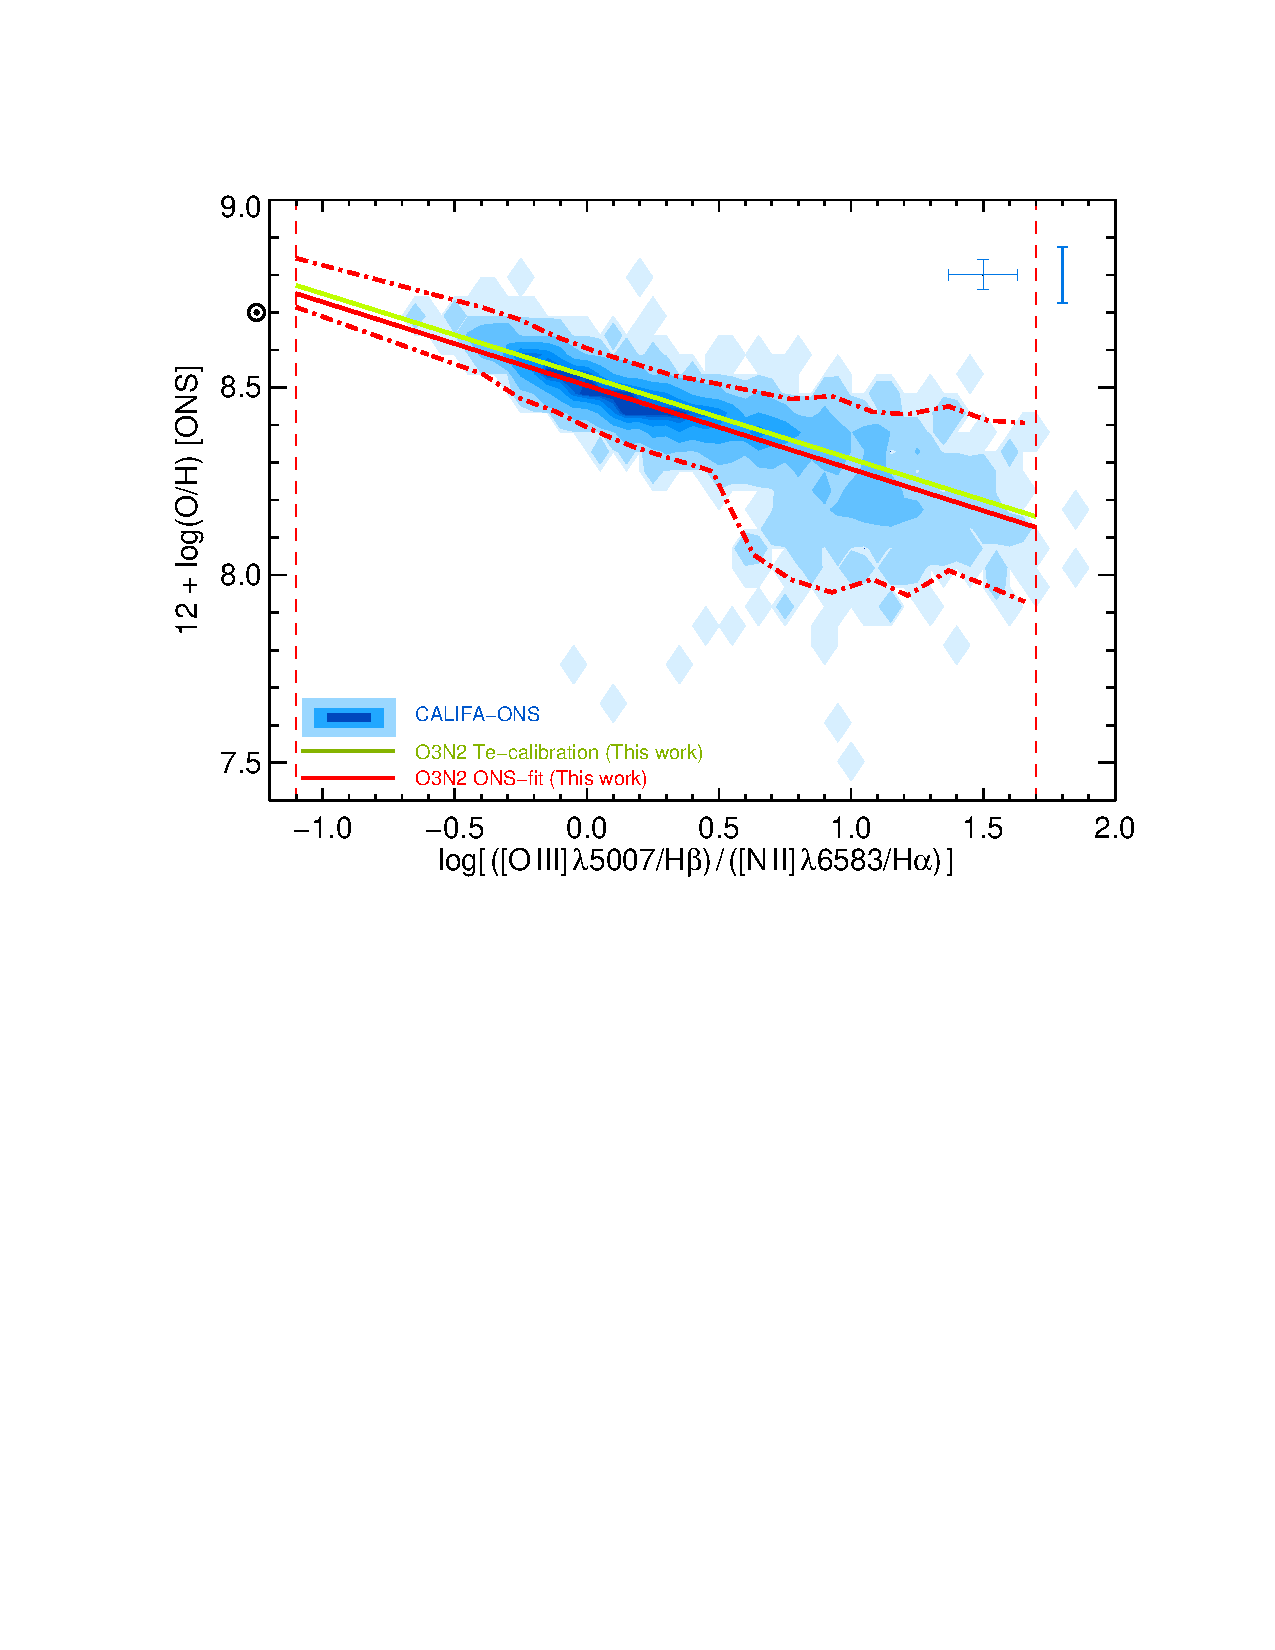
\includegraphics[scale=0.8, trim=2cm 13cm 2cm 3cm, clip]{figuras/O3N2_CALIFA.pdf}
	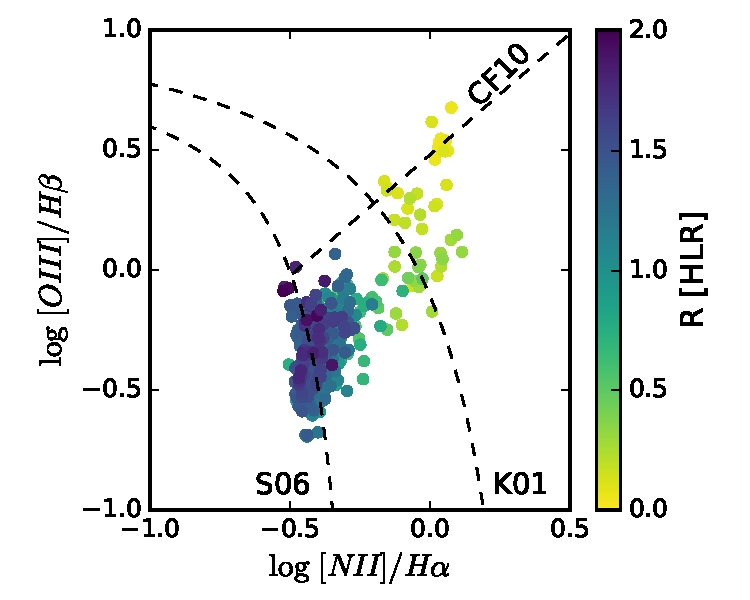
\includegraphics[scale=0.6]{figuras/K0277-BPT.pdf}
	\caption[Diagrama BPT da galáxia NGC2916]
	{Diagrama BPT para as regiões com $S/N > 3$ nas linhas \Hb, \OIII, \Ha e \NII, da galáxia
NGC2916 (objeto CALIFA 277) produzida por um programa como o do exemplo da Figura \ref{fig:BPTprog}.
As cores marcam a distância ao centro da galáxia em unidades do raio que contém metade da luz (HLR). As
linhas são definidas por \citet[][K01]{Kewley.etal.2001a}, \citet[][S06]{Stasinska.etal.2006a} e
\citet[][CF10]{CidFernandes.etal.2010a}.}
	\label{fig:BPTfig}
\end{figure}
%---------------------------- Figure ----------------------------


% End of this chapter
